\chapter{Additional Design Diagrams}
\label{app:diagrams}

\section{Class diagrams}
Each member drew the classes of their own packages (design step A7); every class names the requirements it realises. Table~\ref{tab:design-code} maps these classes to the code.

\begin{sidewaysfigure}
\centering
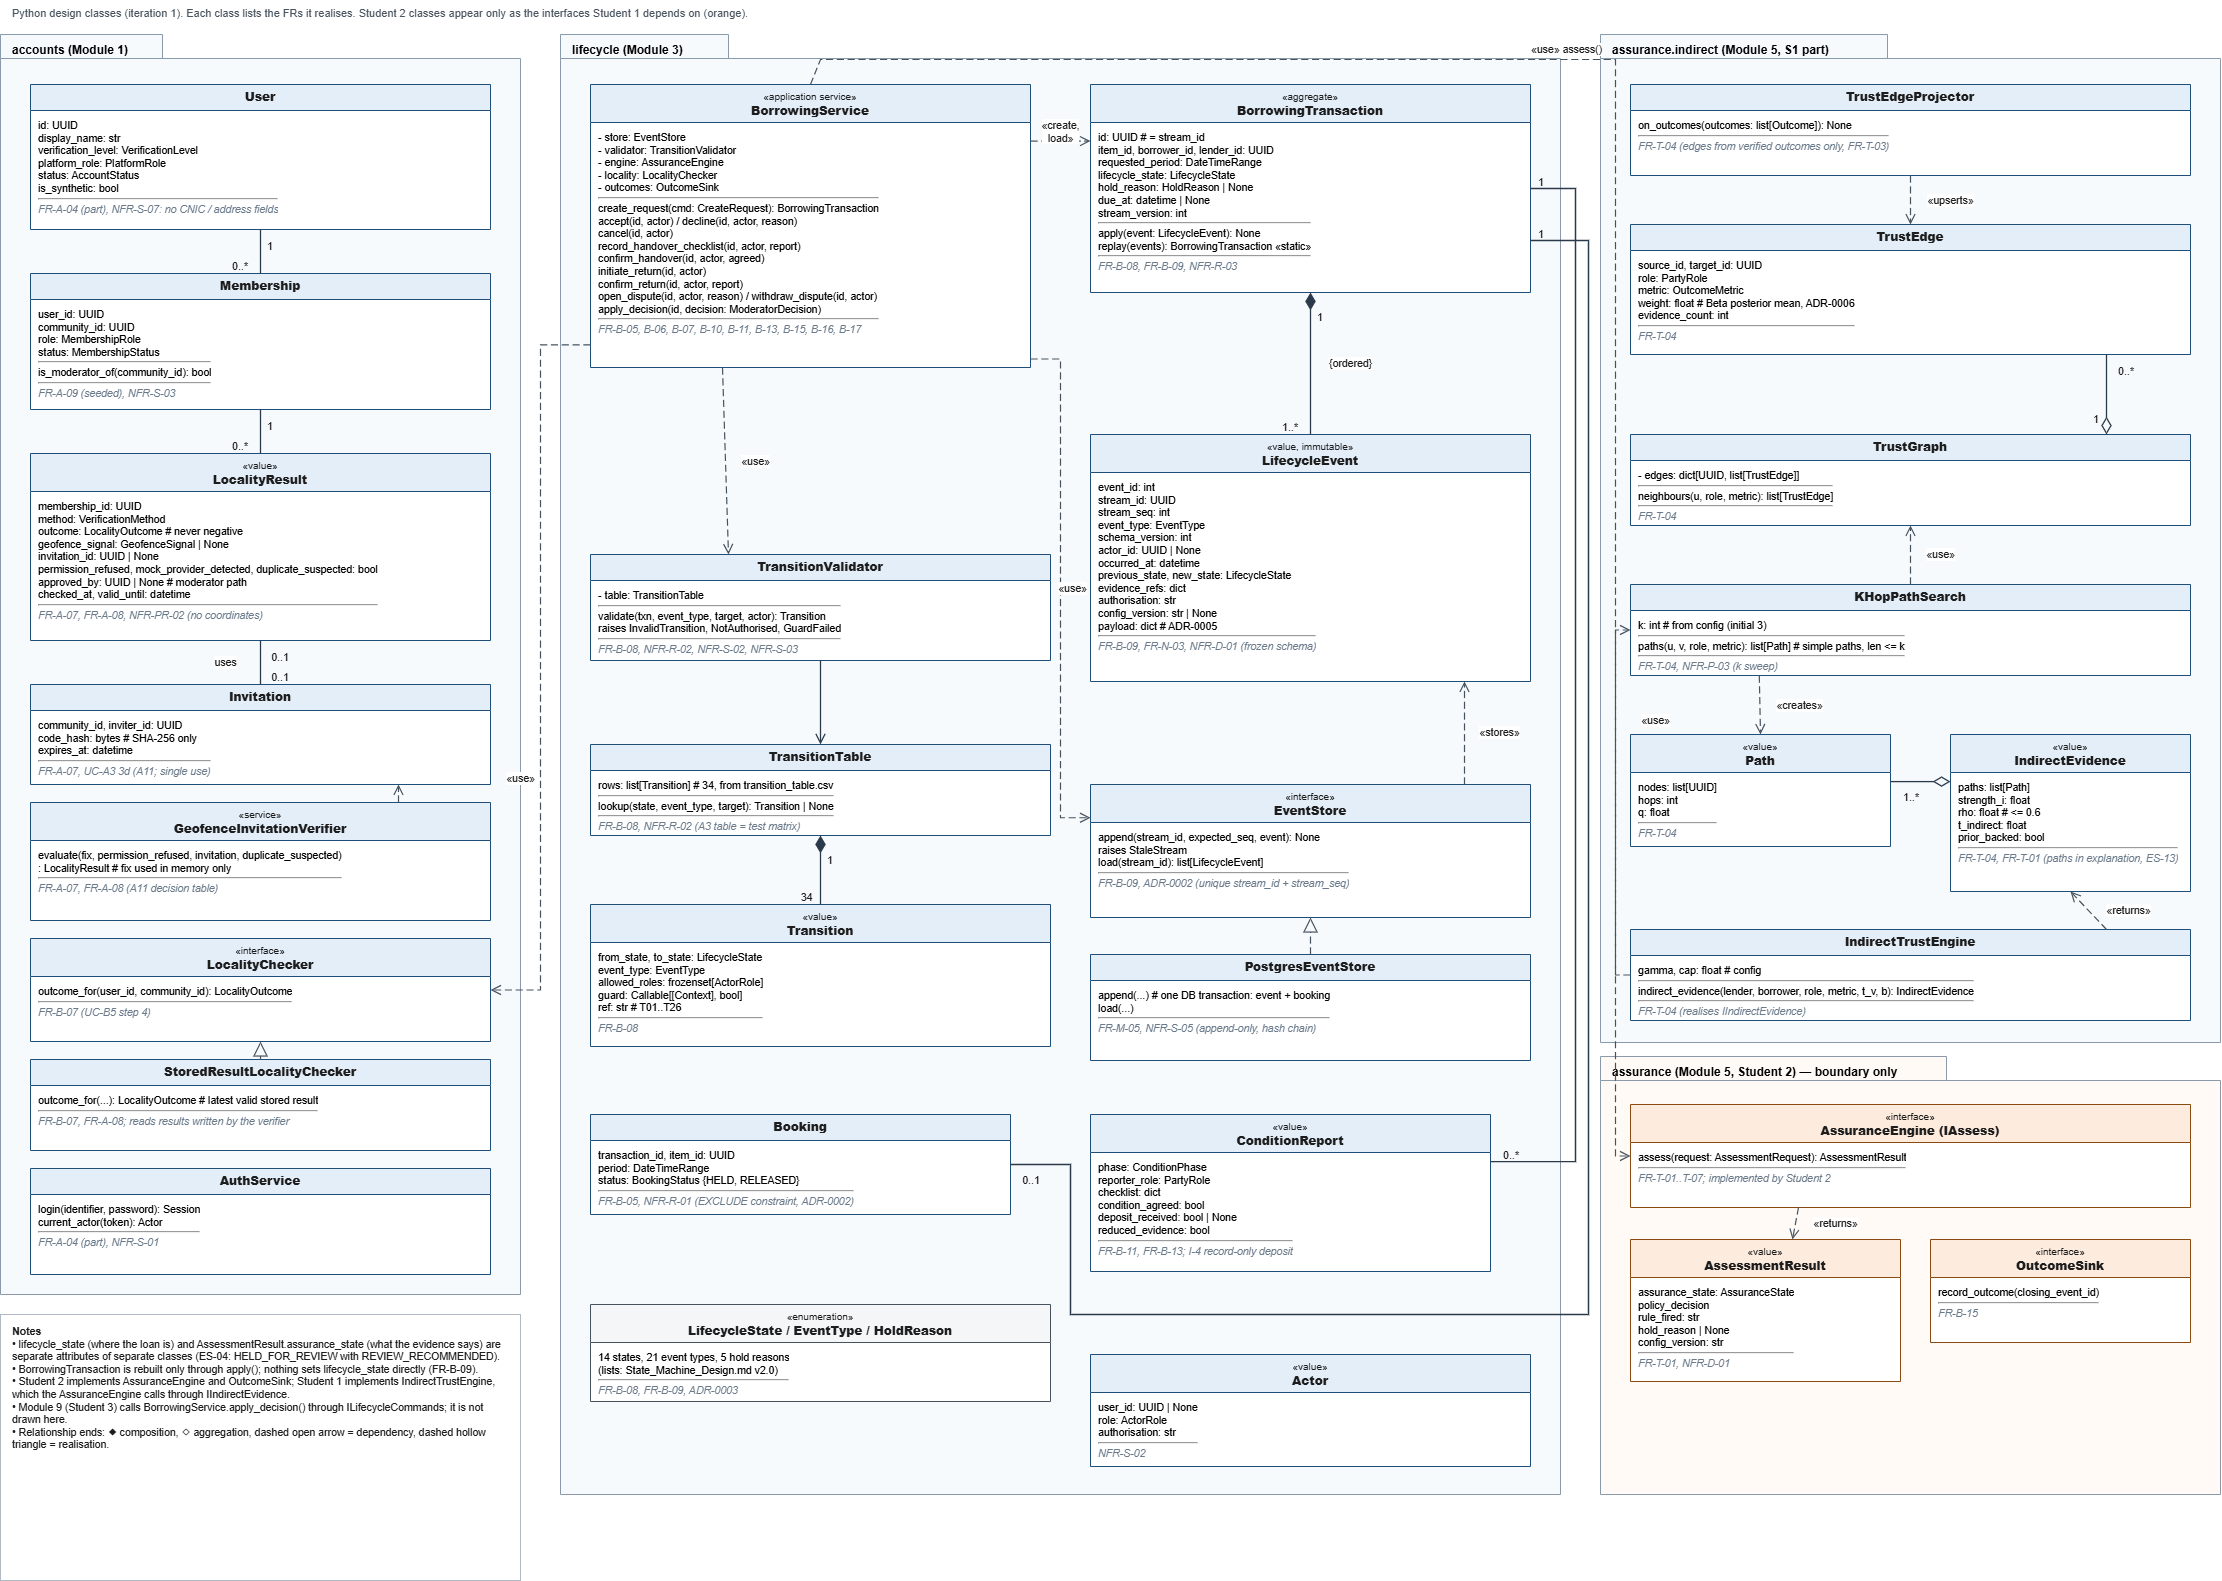
\includegraphics[width=\textheight]{figures/class_s1.png}
\caption{Class diagram, Student 1 packages: accounts and locality, lifecycle and event store, indirect trust}\label{fig:class1}
\end{sidewaysfigure}
\paragraph{Reasoning.} The lifecycle aggregate depends only on the transition table and the ports, so it can be tested without a database; the PostgreSQL event store implements the port. Indirect trust exposes one operation to Student~2's engine. \emph{Serves:} FR-B-05, B-08, B-09, FR-T-04.

\begin{sidewaysfigure}
\centering
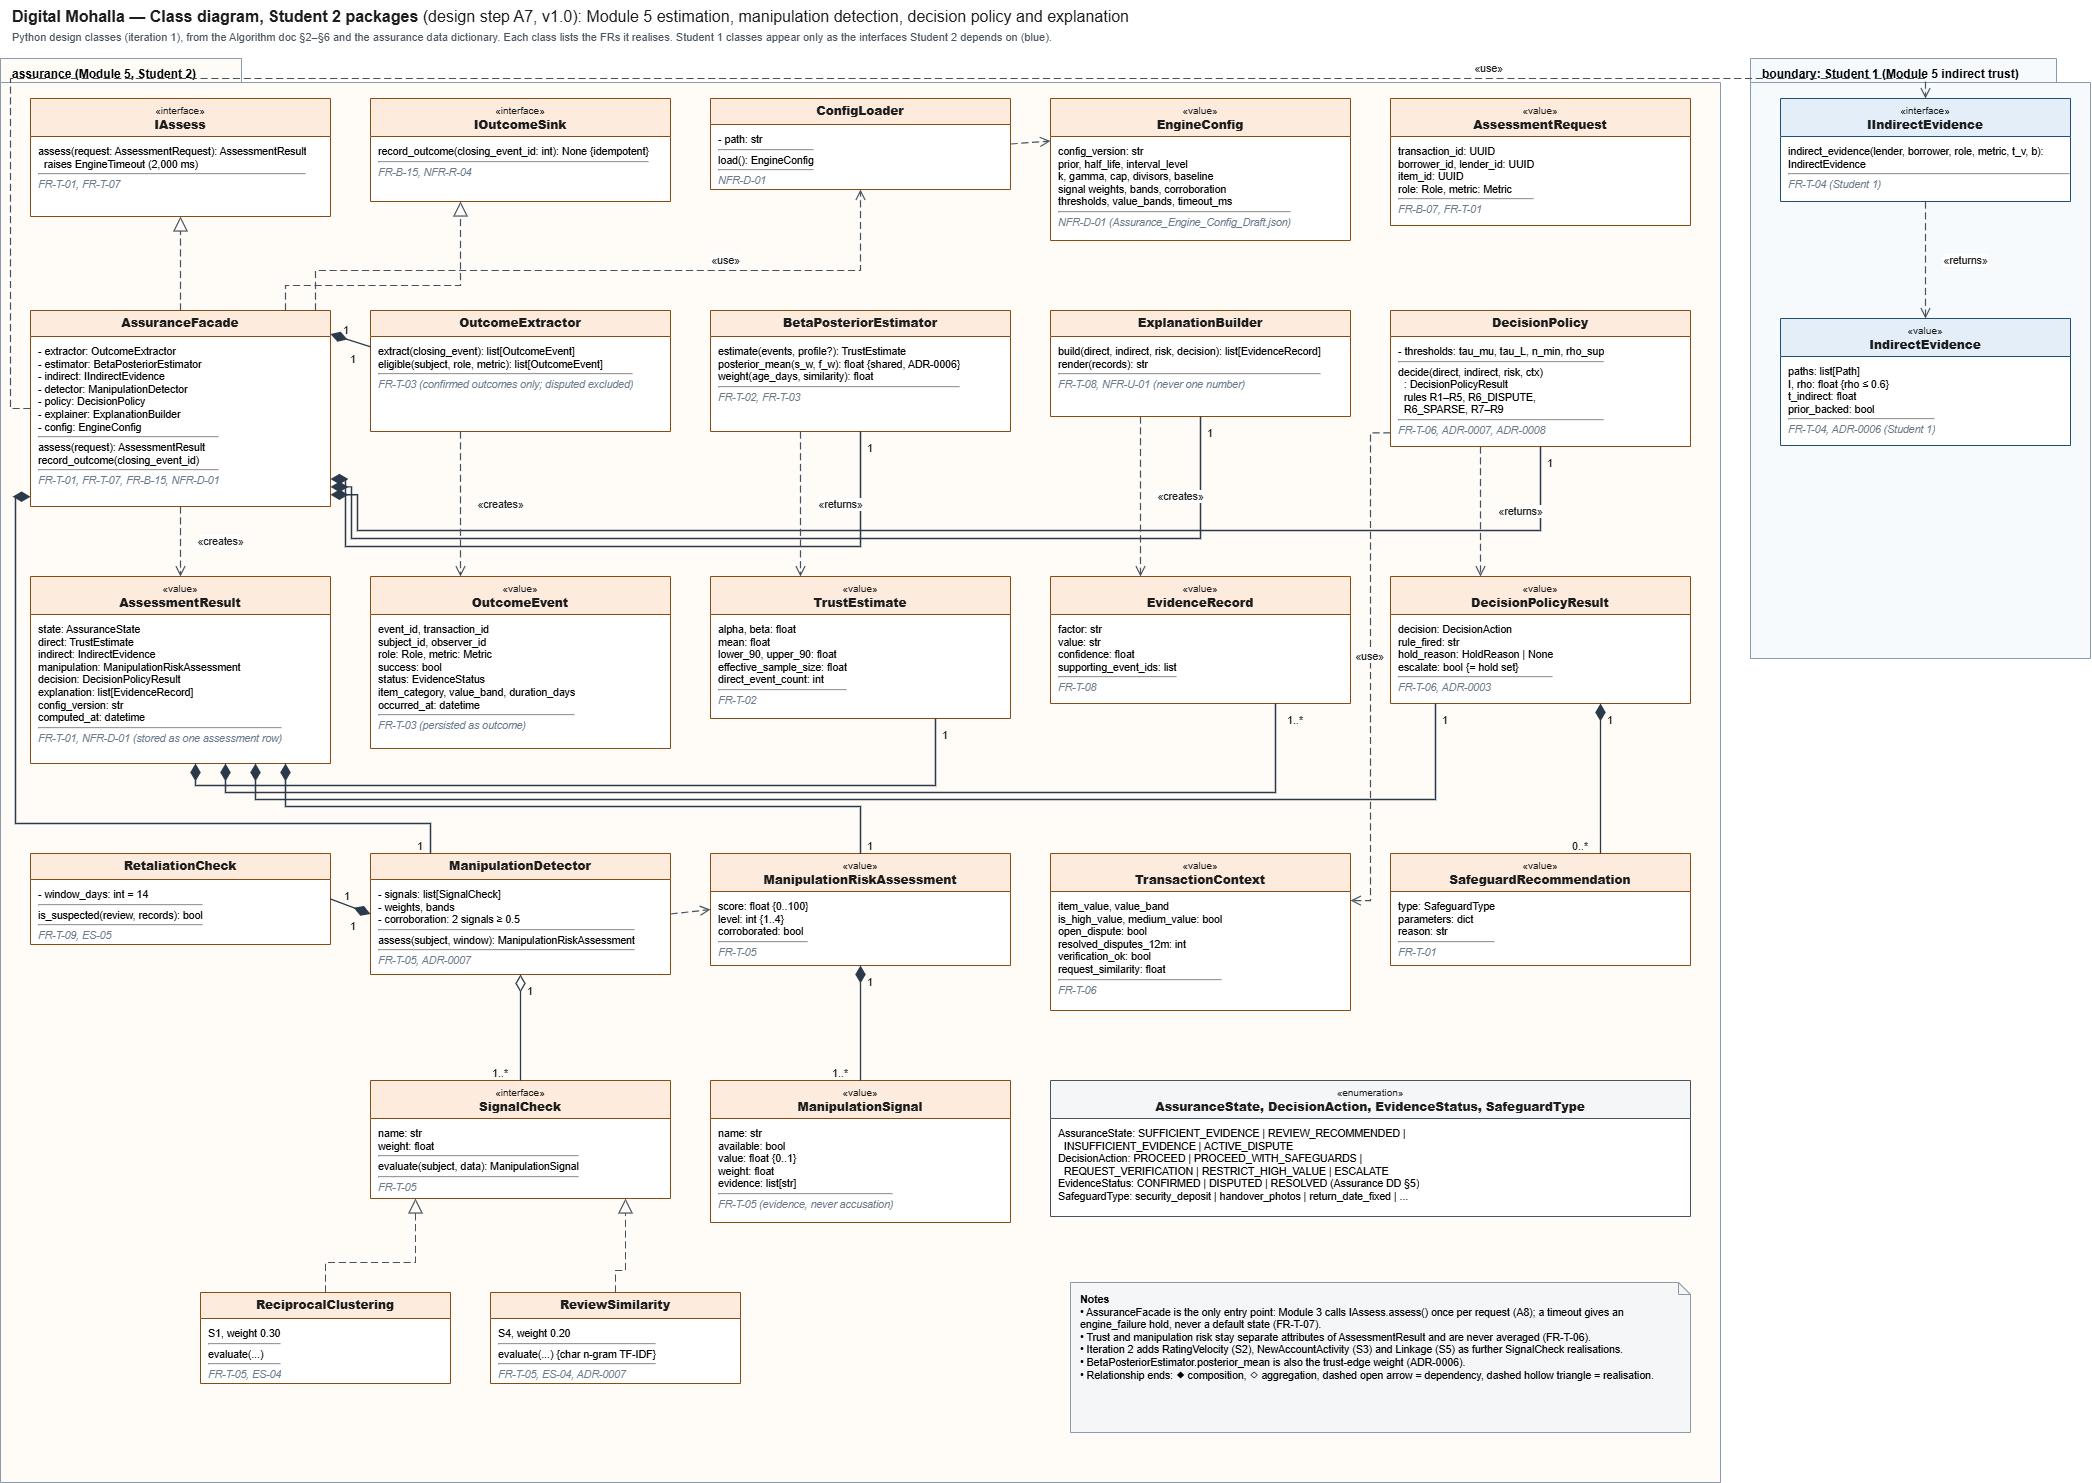
\includegraphics[width=\textheight]{figures/class_s2.png}
\caption{Class diagram, Student 2 packages: estimation, manipulation detection, decision policy and explanation}\label{fig:class2}
\end{sidewaysfigure}
\paragraph{Reasoning.} A single facade runs the pipeline and returns one result object in which trust and manipulation risk are separate attributes, never averaged. Signal checks share one interface so that the Iteration~2 signals (S2, S3, S5) are added without changing the detector. The class named \code{ReciprocalClustering} realises S1, which decision D18 redefined as partner clustering. \emph{Serves:} FR-T-01 to T-08.

\begin{sidewaysfigure}
\centering
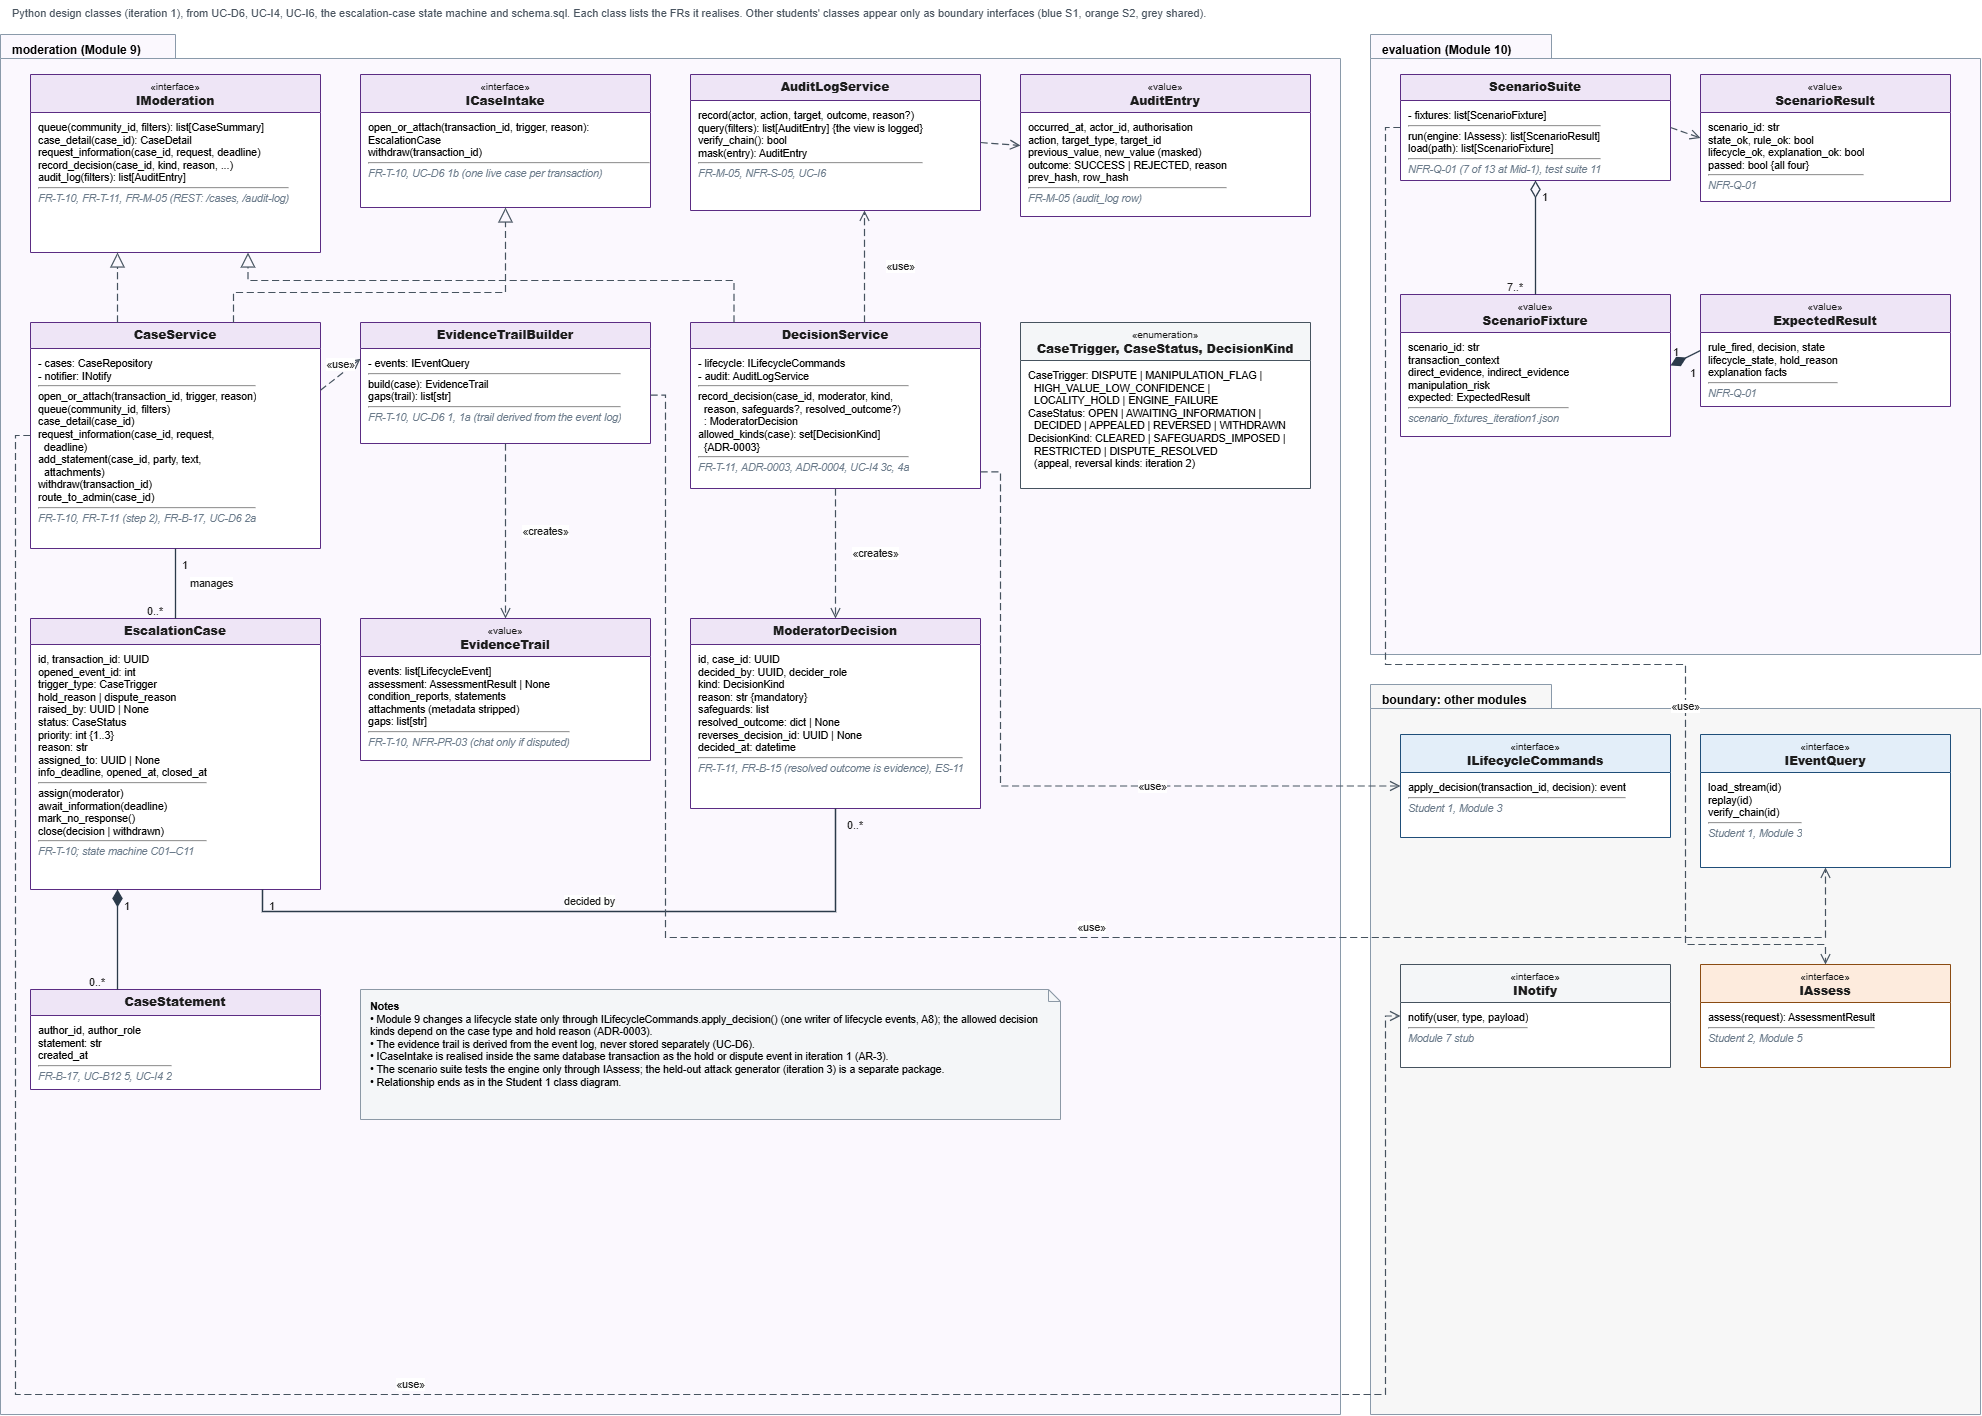
\includegraphics[width=\textheight]{figures/class_s3.png}
\caption{Class diagram, Student 3 packages: cases, decisions and audit (Module 9) and the scenario suite (Module 10)}\label{fig:class3}
\end{sidewaysfigure}
\paragraph{Reasoning.} A moderator decision is a value that the case service turns into exactly one lifecycle command, so moderation cannot bypass the transition rules. \emph{Serves:} FR-T-10, FR-T-11, FR-M-05.

\section{Sequence (b): handover and return to evidence}
\begin{sidewaysfigure}
\centering
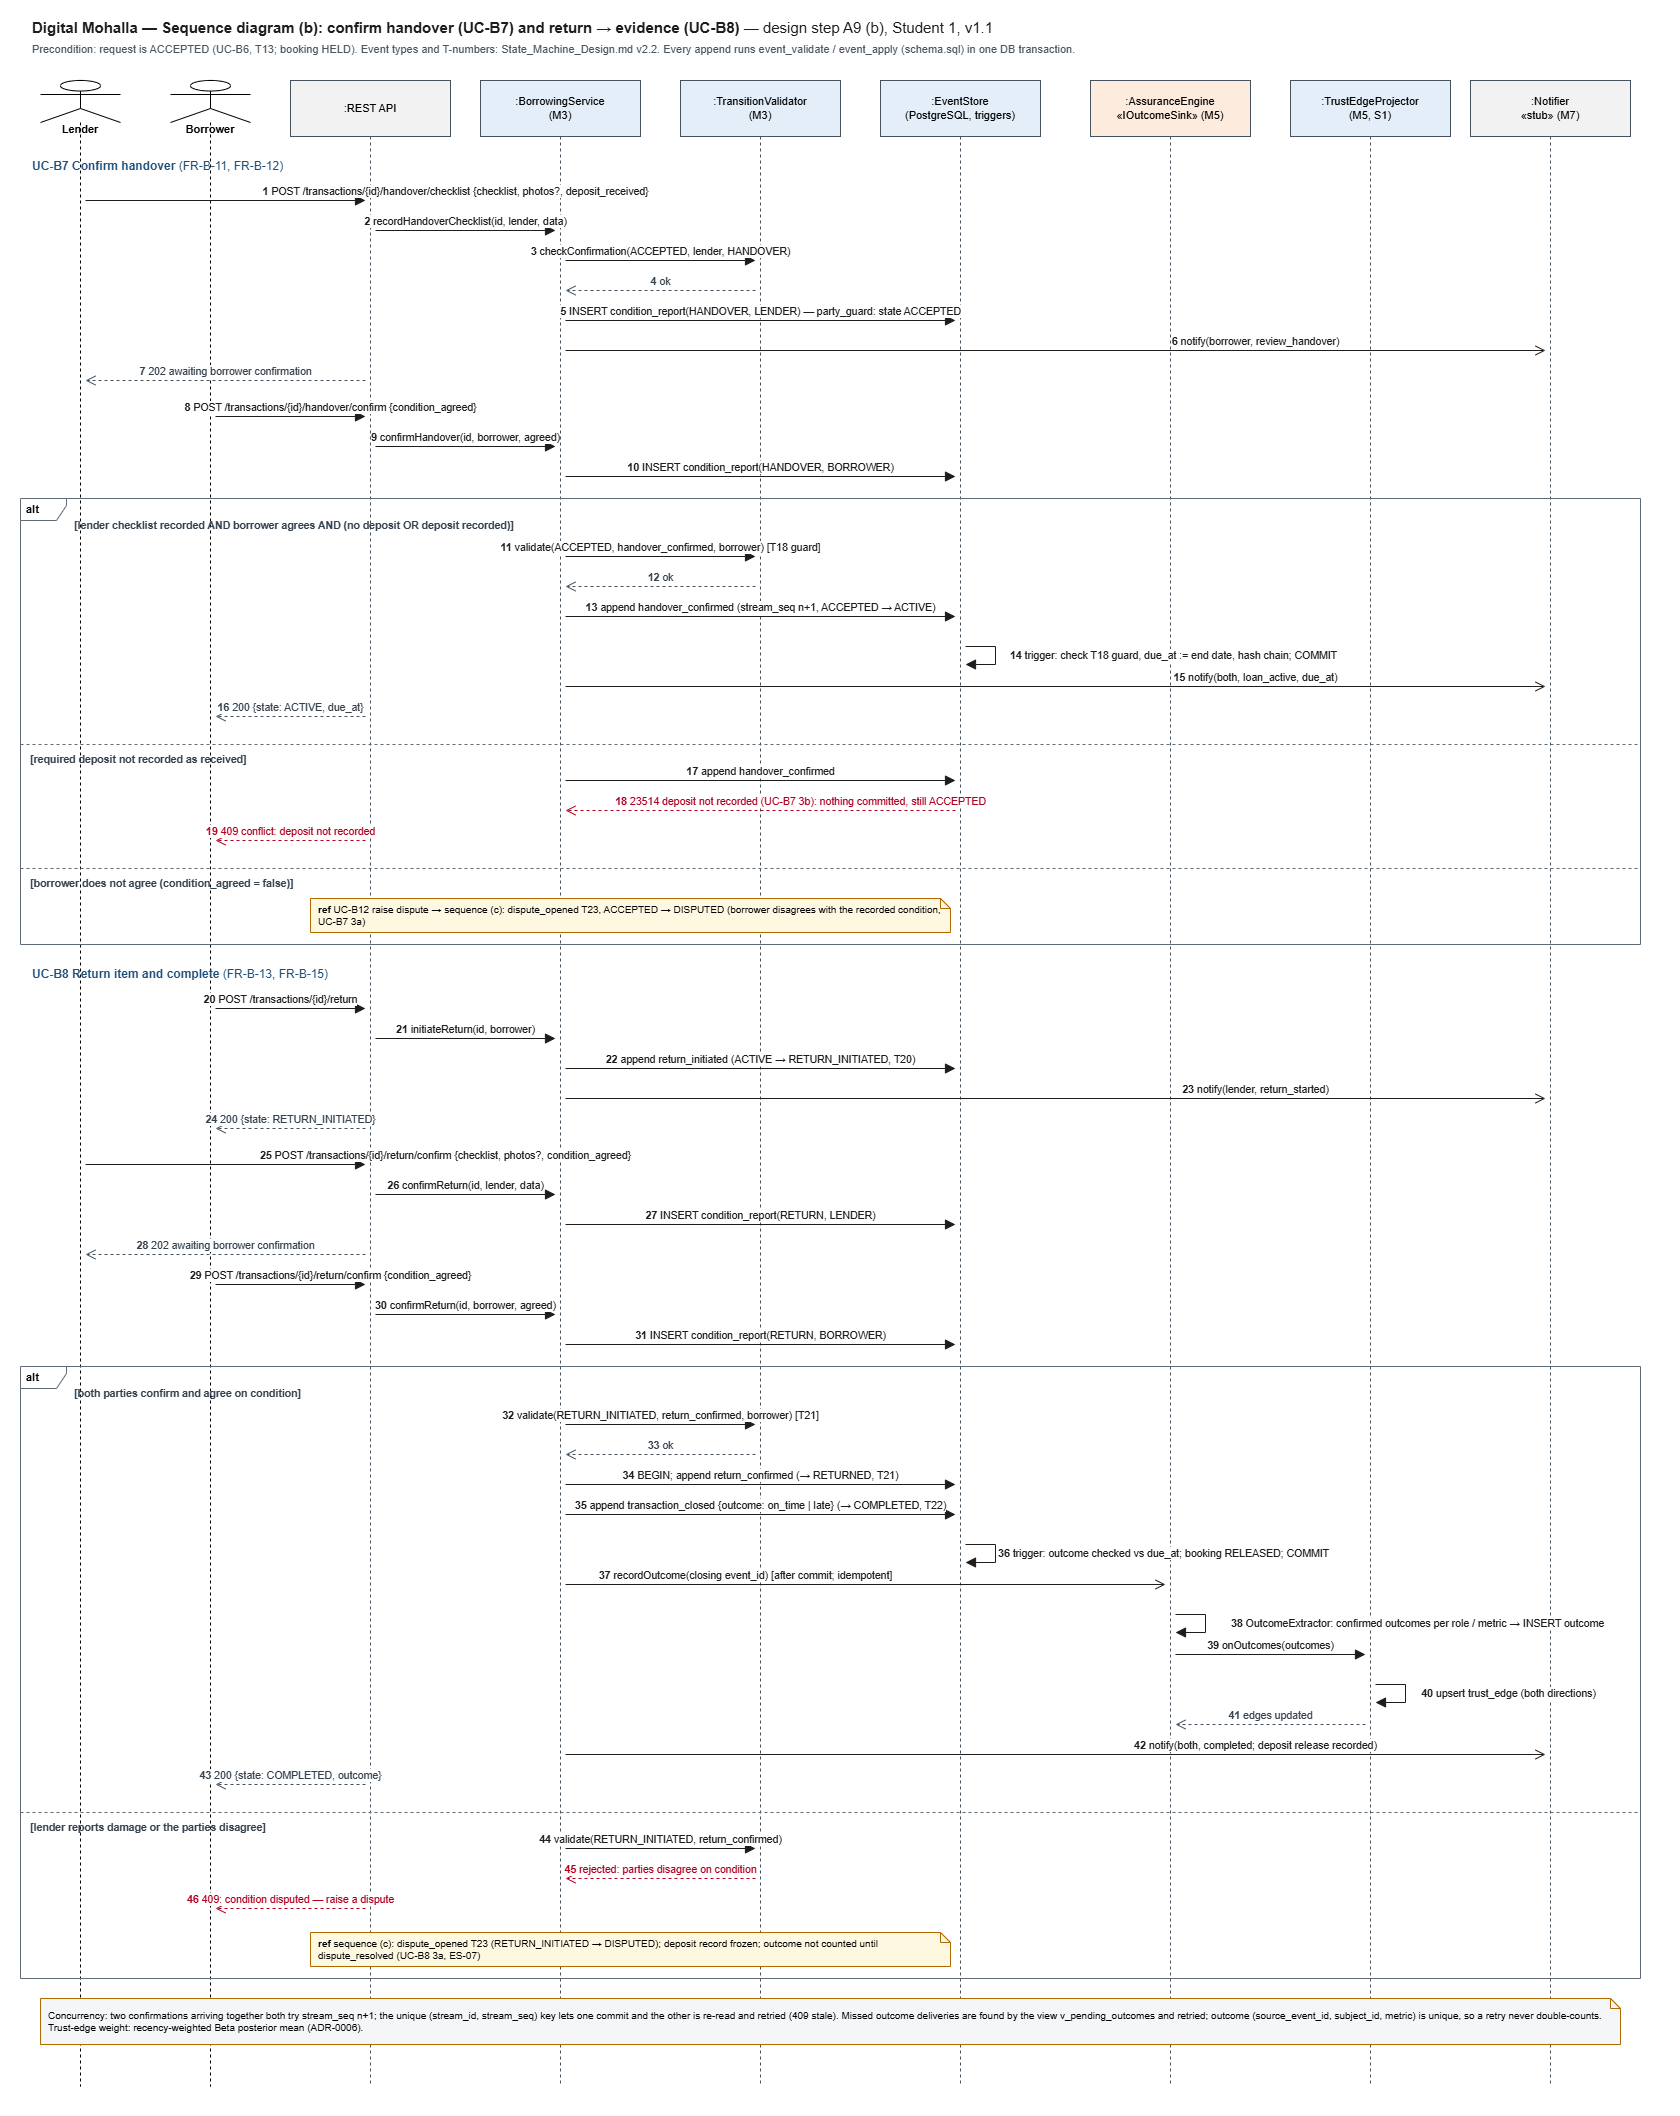
\includegraphics[width=\textheight]{figures/seq_b.png}
\caption{Sequence (b): dual confirmation of handover and return, then outcome to the engine (UC-B7, B8)}\label{fig:seqb}
\end{sidewaysfigure}
\paragraph{Reasoning.} An outcome is written only after both parties have confirmed, which is what makes it ``verified'' evidence (FR-T-03); the close hook writes the outcomes and refreshes the affected trust edges in the same database transaction as \code{transaction\_closed}. \emph{Owner:} S1.

\section{Wireframes}
The wireframes (design step A12, S3) were drawn from the HCI analysis; every screen that shows an assurance state shows its evidence (NFR-U-01). The built screens follow them.

\begin{figure}[H]
\centering
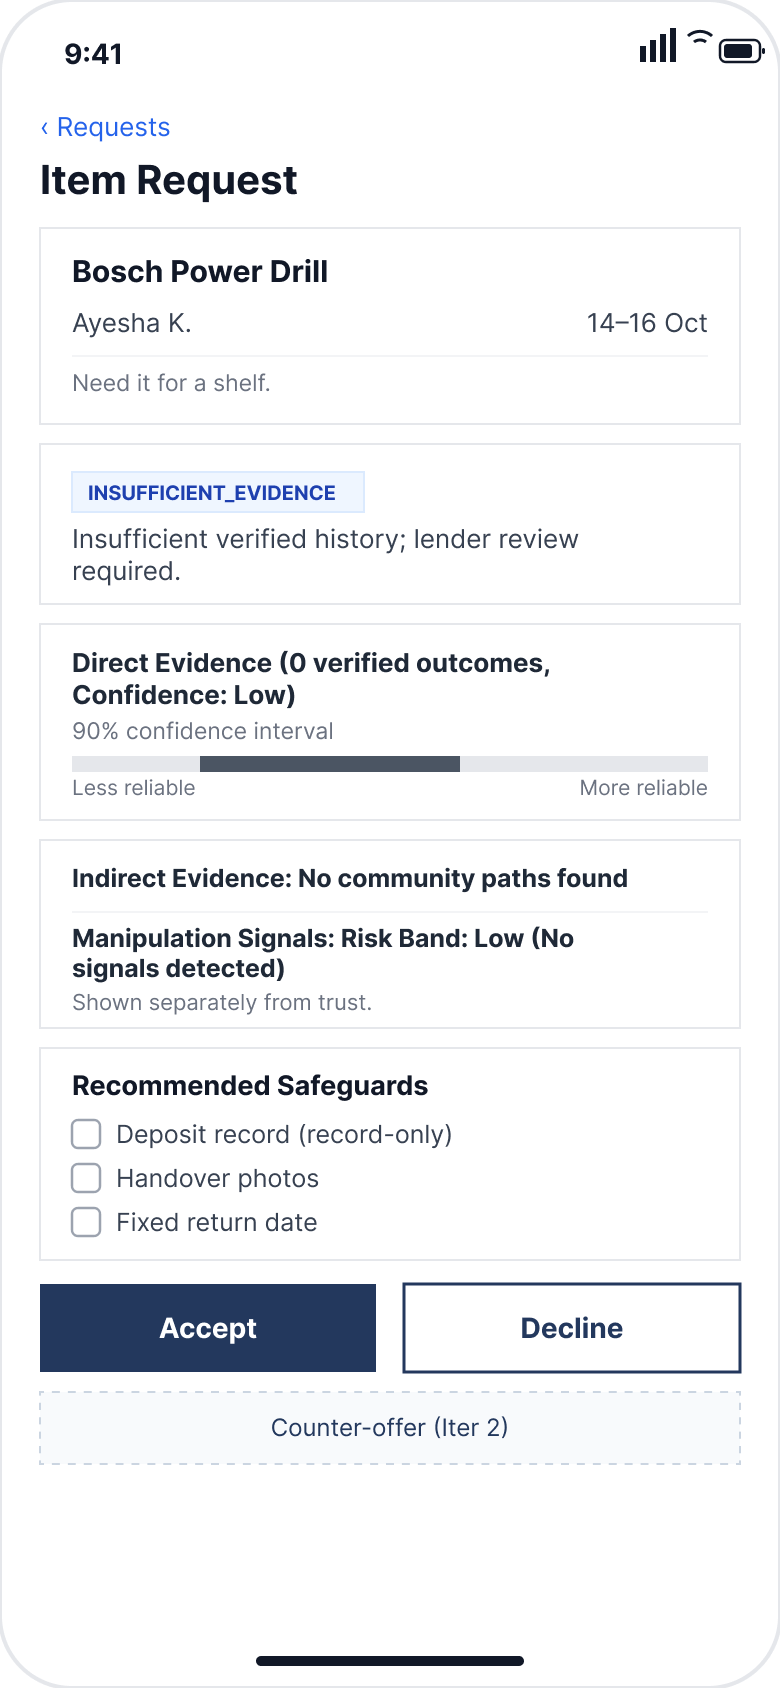
\includegraphics[width=0.45\textwidth]{figures/wf_W1_Lender_Request_Assurance.png}\hfill
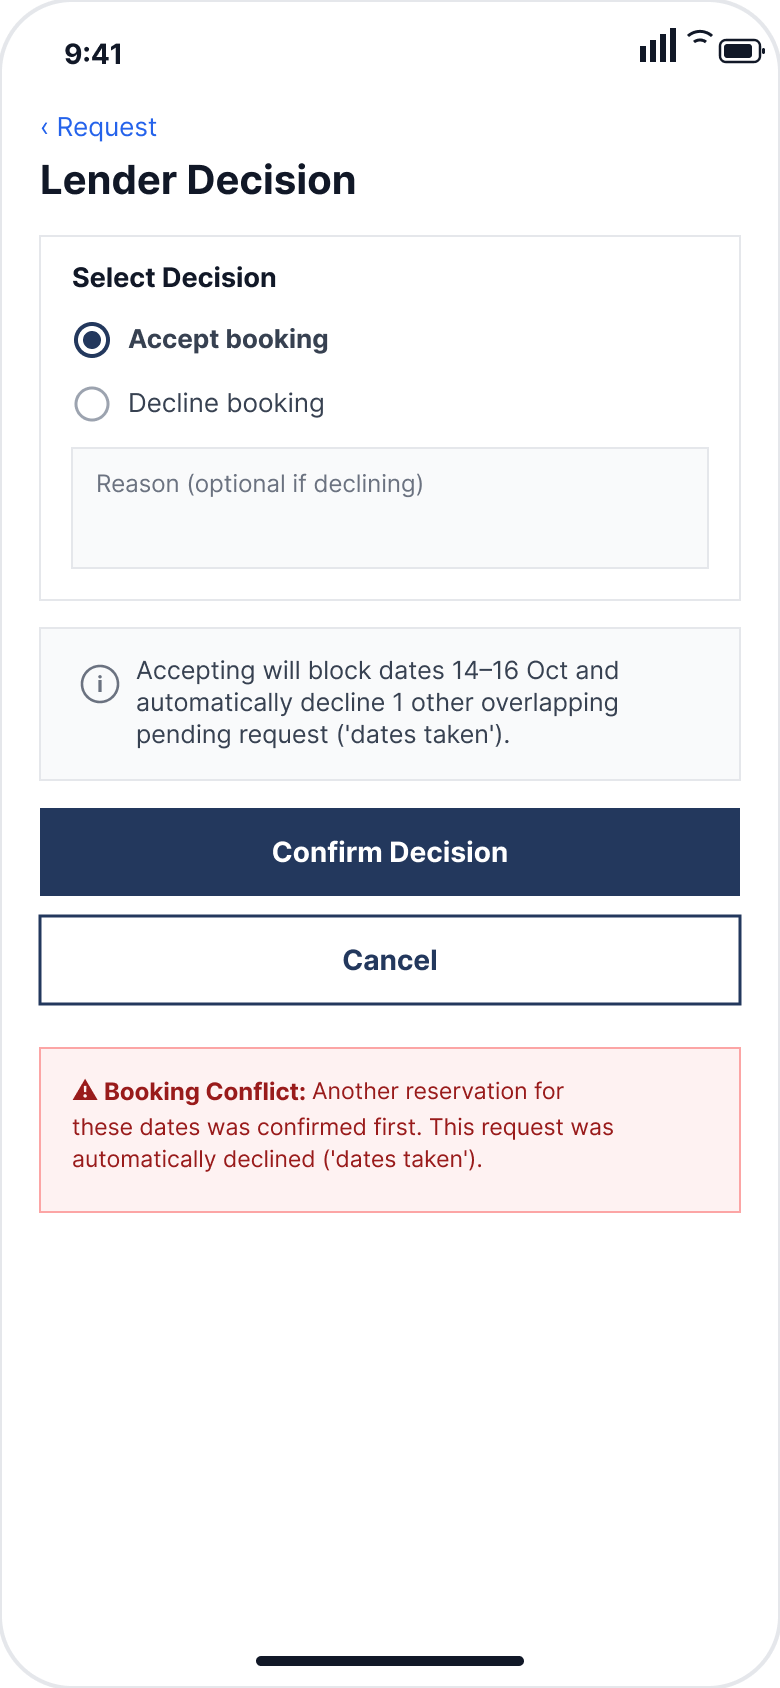
\includegraphics[width=0.45\textwidth]{figures/wf_W2_Lender_Decision_Conflict.png}
\caption{W1 lender request with assurance summary; W2 lender decision and date conflict}\label{fig:w12}
\end{figure}
\begin{figure}[H]
\centering
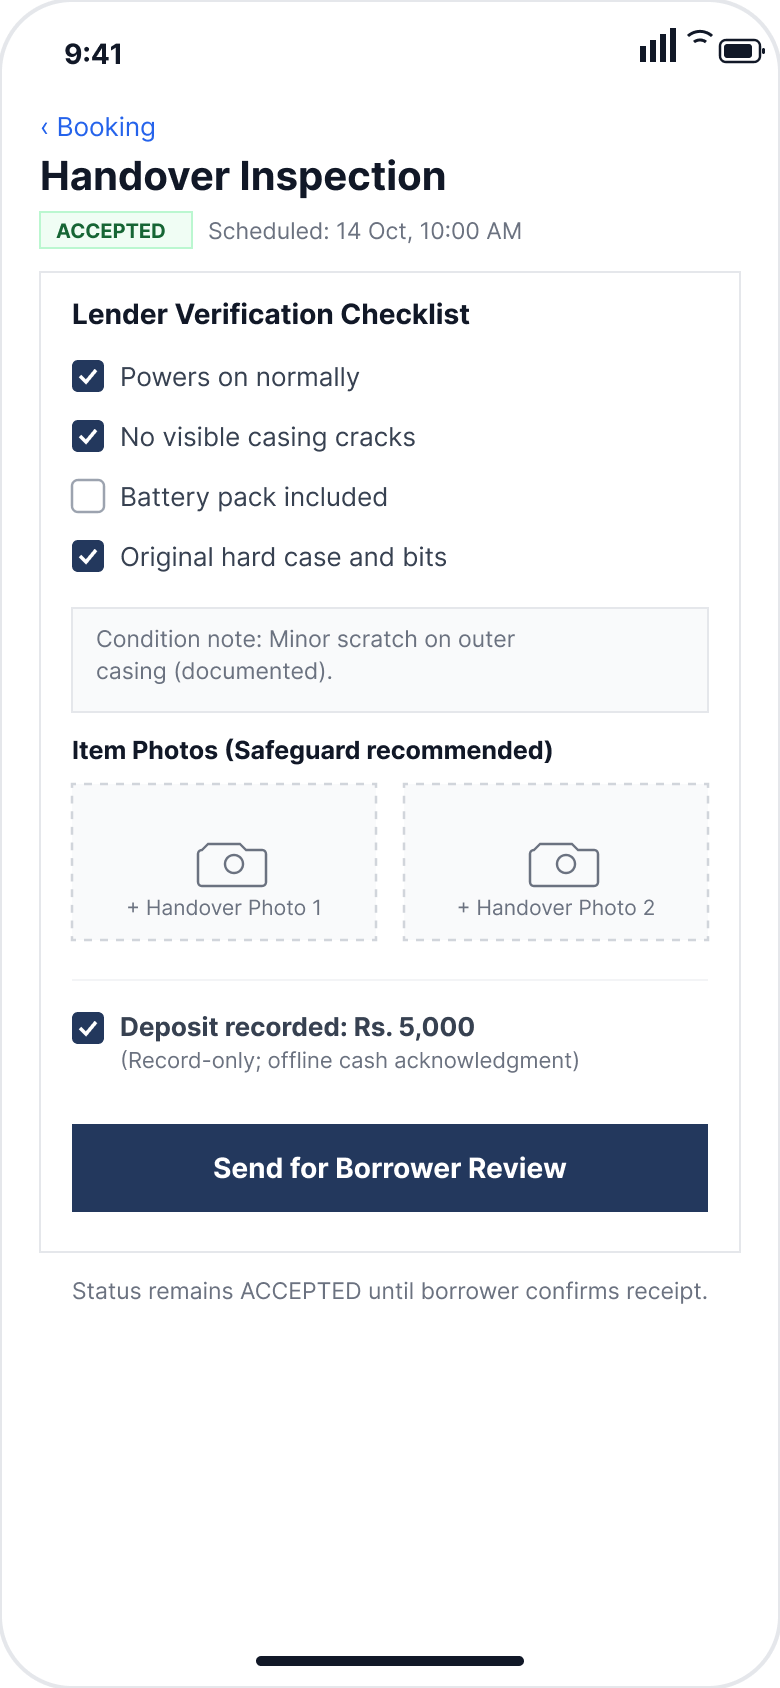
\includegraphics[width=0.45\textwidth]{figures/wf_W3a_Handover_Inspection_Lender.png}\hfill
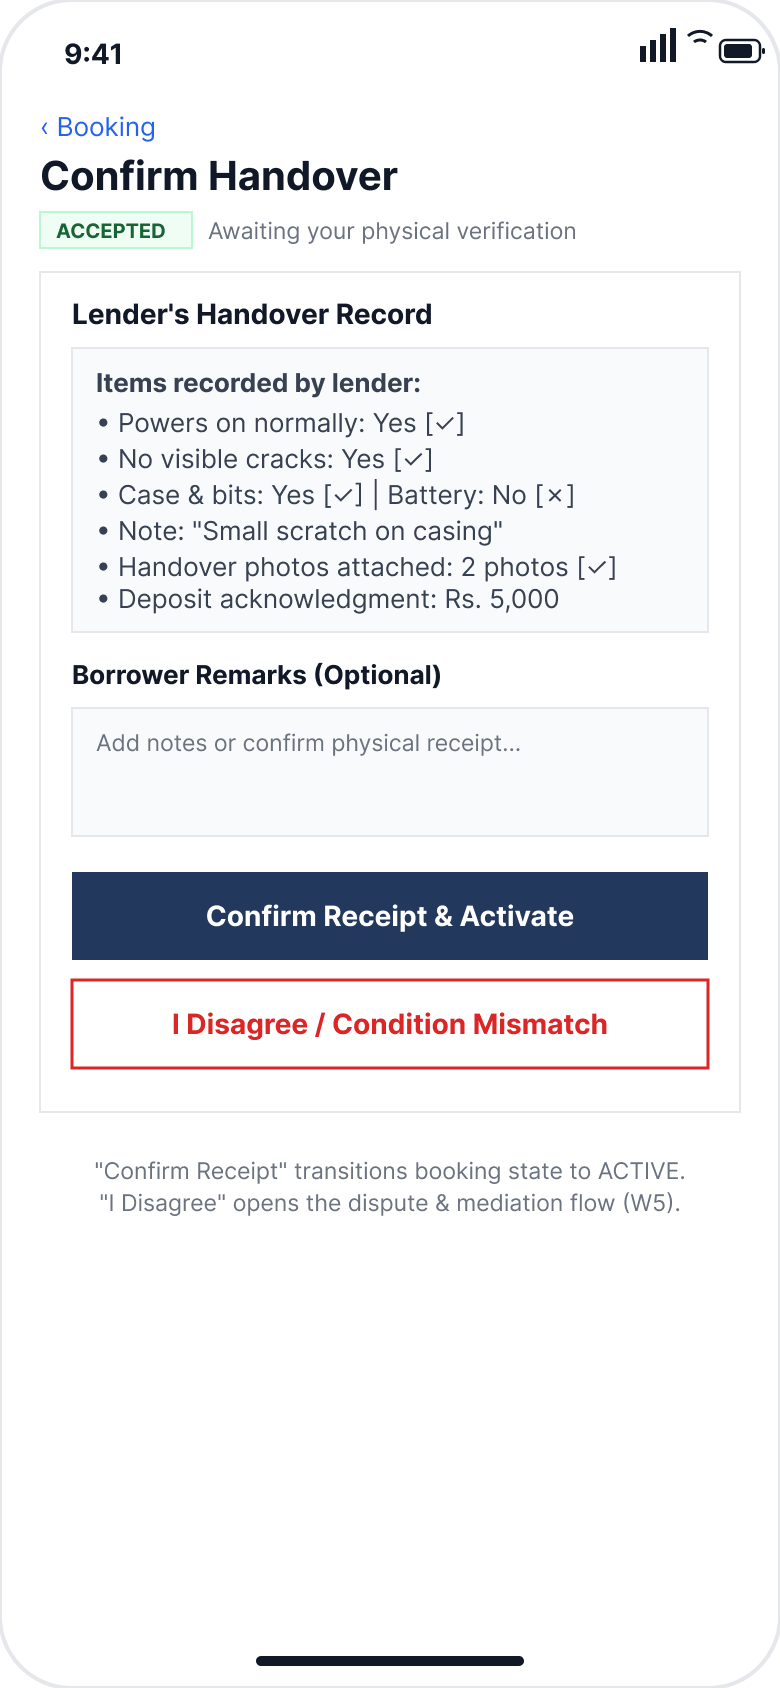
\includegraphics[width=0.45\textwidth]{figures/wf_W3b_Handover_Confirmation_Borrower.png}
\caption{W3a handover inspection (lender); W3b handover confirmation (borrower)}\label{fig:w3}
\end{figure}
\begin{figure}[H]
\centering
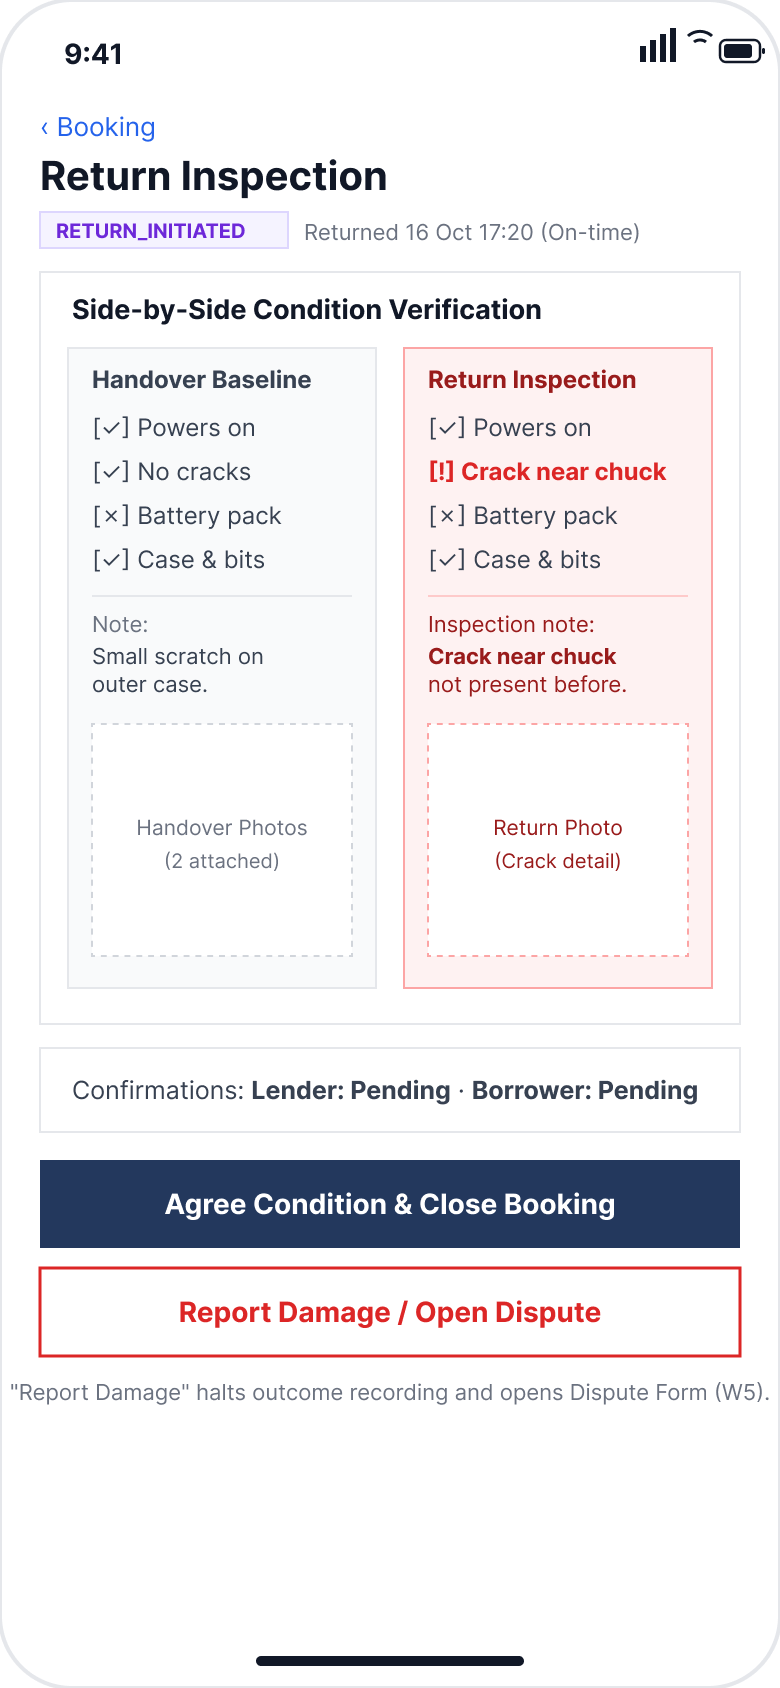
\includegraphics[width=0.45\textwidth]{figures/wf_W4_Return_Inspection_Comparison.png}\hfill
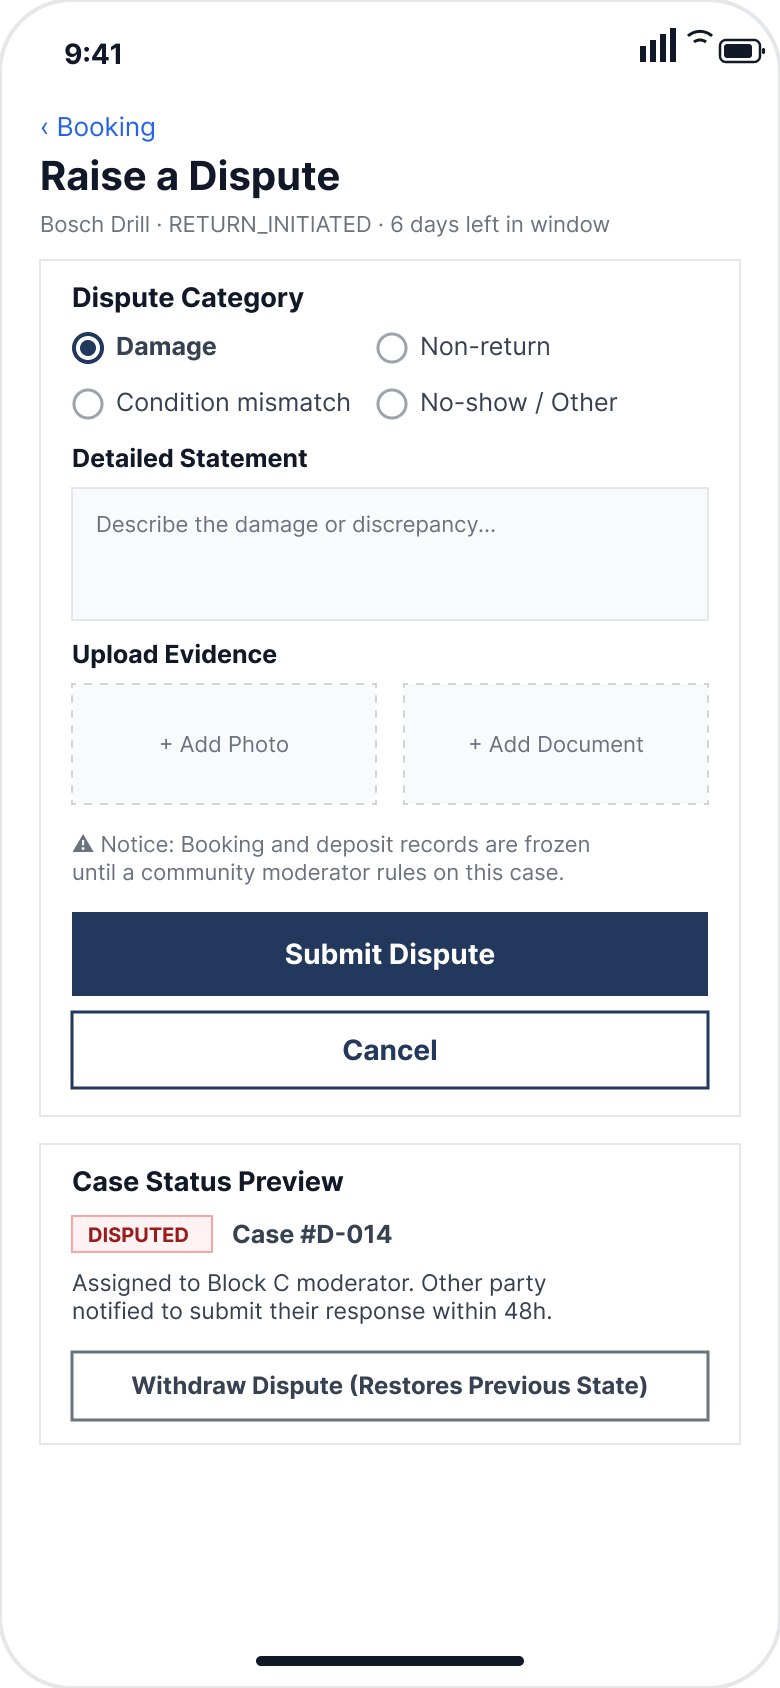
\includegraphics[width=0.45\textwidth]{figures/wf_W5_Dispute_Form_Progress.png}
\caption{W4 return inspection; W5 dispute form and progress}\label{fig:w45}
\end{figure}
\begin{figure}[H]
\centering
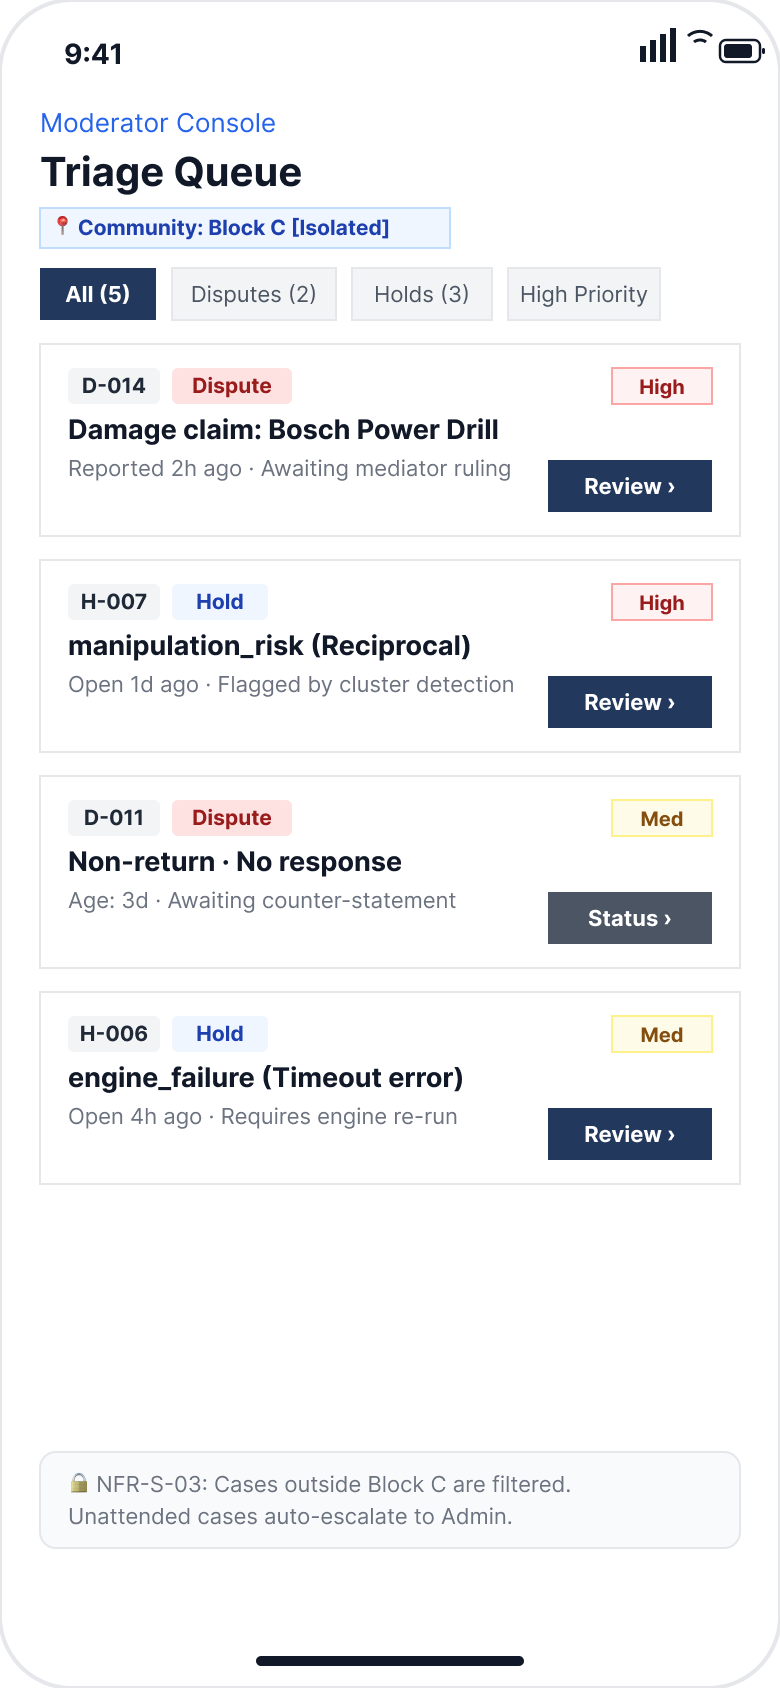
\includegraphics[width=0.45\textwidth]{figures/wf_W6_Moderator_Queue_Mobile.png}\hfill
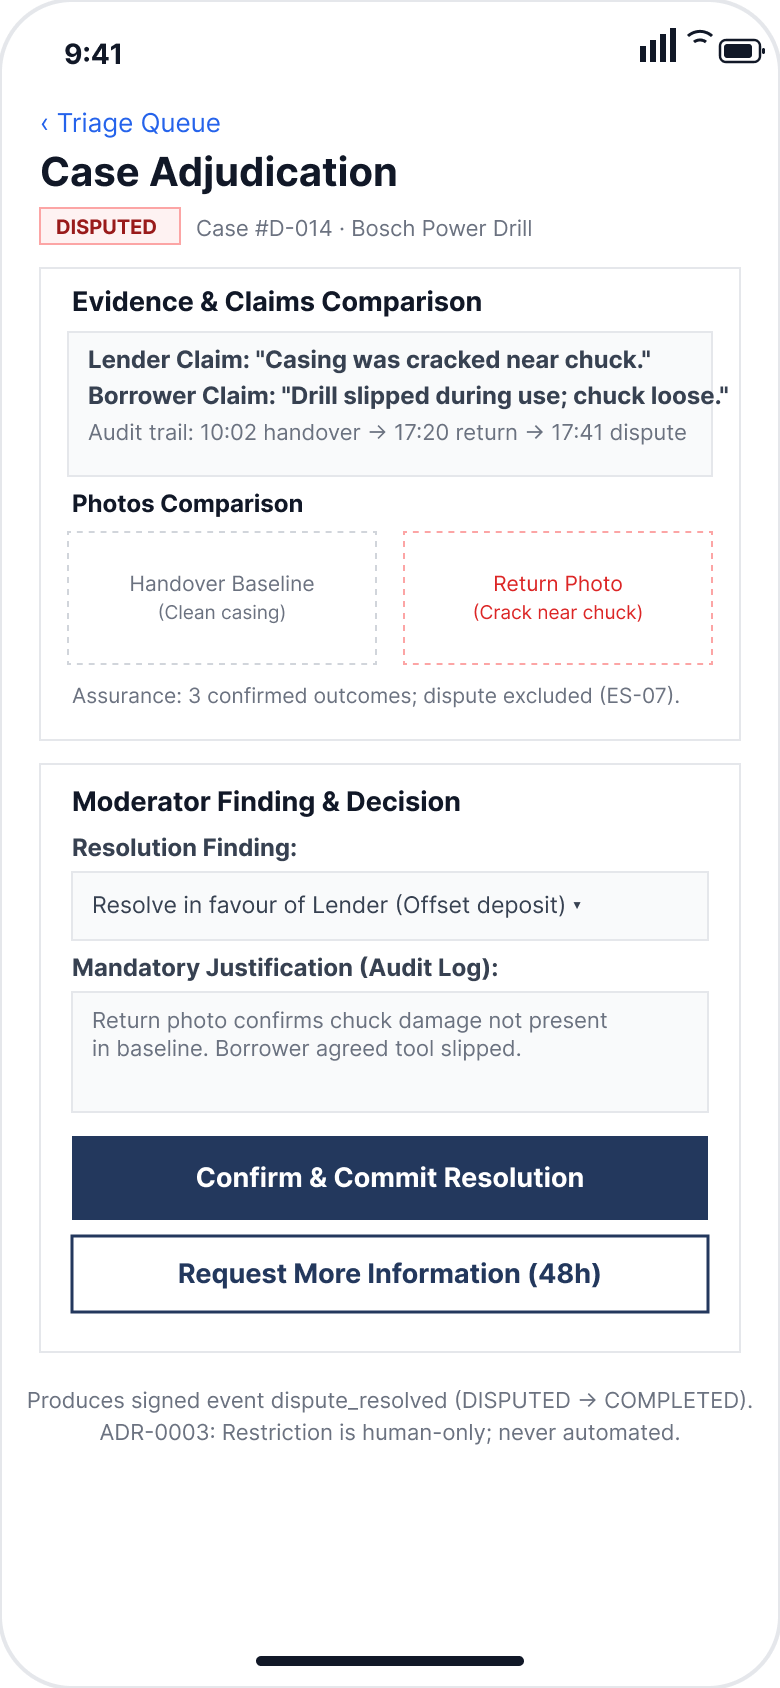
\includegraphics[width=0.45\textwidth]{figures/wf_W7_Moderator_Case_Adjudication_Mobile.png}
\caption{W6 moderator queue; W7 case adjudication}\label{fig:w67}
\end{figure}
